% !TEX program = xelatex
\documentclass[11pt,a4paper]{article}

\usepackage{fontspec}
\usepackage[a4paper,margin=2.4cm]{geometry}
\usepackage{amsmath,amssymb,mathtools}
\usepackage{siunitx}
\usepackage{booktabs,tabularx}
\usepackage{enumitem}
\usepackage{caption}
\usepackage{microtype}
\usepackage{tikz}
\usetikzlibrary{arrows.meta,patterns,decorations.pathmorphing,calc}
\usepackage[colorlinks=true,linkcolor=teal!70!black,citecolor=teal!70!black,urlcolor=teal!70!black]{hyperref}

\renewcommand{\contentsname}{Índice}
\renewcommand{\figurename}{Figura}
\renewcommand{\tablename}{Tabla}
\renewcommand{\refname}{Referencias}
\renewcommand{\abstractname}{Resumen}
\sisetup{output-decimal-marker={,}, group-separator={\,}, per-mode=symbol, range-phrase={--}}
\setlength{\emergencystretch}{3em}
\setlist{itemsep=2pt,topsep=4pt}

\newcommand{\dd}{\mathrm{d}}
\newcommand{\psat}{p_{\mathrm{sat}}}
\newcommand{\Tsat}{T_{\mathrm{sat}}}
\newcommand{\hfg}{h_{fg}}
\newcommand{\mdot}{\dot m}
\newcommand{\Qdot}{\dot Q}
\newcommand{\Wdot}{\dot W}
\newcommand{\en}[1]{\textit{(#1)}}

\newenvironment{nota}{\par\smallskip\noindent\begin{minipage}{\linewidth}\small\itshape}{\end{minipage}\par\smallskip}

\title{\textbf{Física del evaporador inercial de oscilador abierto}\\[4pt]
\large Principios, ecuaciones y órdenes de magnitud de un pistón líquido que genera, comprime y expulsa vapor}
\author{Miguel Ángel Rodríguez García}
\date{Octubre de 2026}

\begin{document}
\maketitle

\begin{abstract}
\noindent Este documento desarrolla, con nivel de detalle de especialista, la física de un evaporador inercial de oscilador abierto: una columna de agua de varias toneladas que oscila entre un tubo alto, cuya parte superior contiene vapor, y un tanque lateral con un colchón de gas. Al caer, la columna deja tras de sí un espacio a baja presión en el que el agua caliente se evapora de forma súbita; al subir, comprime y calienta ese vapor; y al llegar arriba lo expulsa a través de una válvula. Se derivan la dinámica de la columna con inercia variable a partir de la ecuación de Bernoulli no estacionaria y de la formulación lagrangiana; la termodinámica del colchón de gas y del espacio de vapor como volúmenes de control abiertos; la cinética y la limitación térmica de la evaporación y la condensación; la transferencia de calor a las paredes; el flujo compresible de expulsión; y los balances de energía y exergía que acotan el coeficiente de rendimiento. Cada mecanismo se acompaña de órdenes de magnitud calculados para un caso de referencia ilustrativo y de un análisis de qué mecanismo domina y por qué.

\smallskip\noindent\textbf{Alcance.} La arquitectura sigue la descripción pública de Hydram Dynamics \cite{hydramweb,hydramtech,hydramtcw}. Las geometrías, parámetros y resultados numéricos son propios e ilustrativos: no describen ni predicen el equipo de Hydram.
\end{abstract}

\tableofcontents
\newpage

%=====================================================================
\section{Descripción del proceso}
%=====================================================================

\subsection{Arquitectura}

El sistema (figura~\ref{fig:esquema}) consta de cuatro elementos:
\begin{enumerate}
  \item Un \textbf{tubo alto} vertical \en{high pipe} de diámetro $D_h$ y altura $H$, cerrado arriba salvo por la válvula de expulsión. Por encima del nivel del líquido $z$ hay un espacio de vapor de volumen $V_s$.
  \item Un \textbf{tanque lateral} ancho \en{side tank} de sección $A_t \gg A_h$, conectado al tubo alto por abajo, con un \textbf{colchón de gas} \en{gas cushion} de volumen $V_g$ sobre su superficie libre.
  \item Una \textbf{válvula antirretorno de expulsión} en lo alto del tubo, que descarga al colector de vapor \en{steam header} a presión $p_{\mathrm{out}}$.
  \item Un \textbf{intercambiador de calor residual} en la parte alta del tubo, que aporta el calor necesario para compensar el enfriamiento evaporativo y mantiene el agua y las paredes a una temperatura $T_b$.
\end{enumerate}
Un actuador mantiene la oscilación aplicando una pequeña sobrepresión en el sentido del movimiento: \emph{``aumentar alternativamente la presión detrás del pistón líquido y disminuirla delante''} \cite{hydramtech}.

\begin{figure}[ht]
\centering
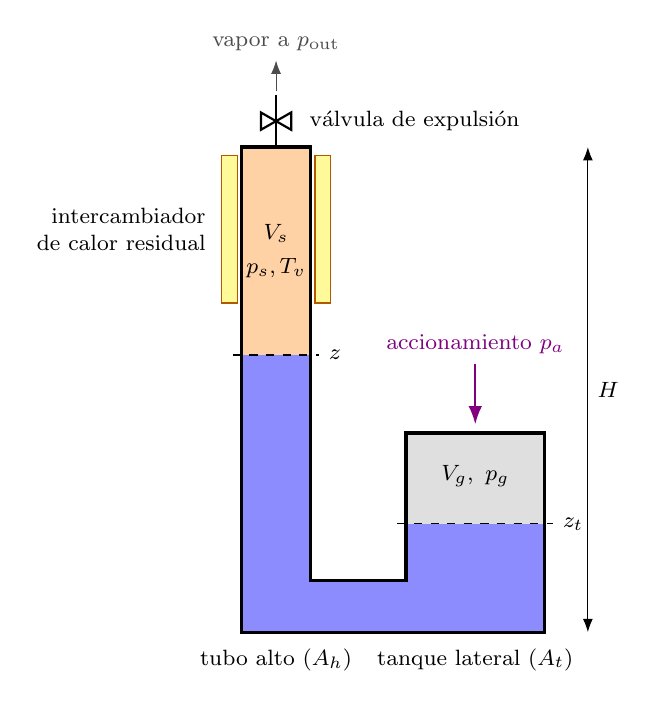
\begin{tikzpicture}[scale=0.55, every node/.style={font=\footnotesize}]
  % liquid
  \fill[blue!45] (0,-1.2) rectangle (7,0);
  \fill[blue!45] (0,0) rectangle (1.6,5.2);
  \fill[blue!45] (3.8,0) rectangle (7,1.3);
  % vapour, gas
  \fill[orange!35] (0,5.2) rectangle (1.6,10);
  \fill[gray!25] (3.8,1.3) rectangle (7,3.4);
  % walls
  \draw[very thick] (0,-1.2) -- (0,10) -- (1.6,10) -- (1.6,0) -- (3.8,0) -- (3.8,3.4) -- (7,3.4) -- (7,-1.2) -- cycle;
  % heat exchanger
  \fill[yellow!40,draw=orange!70!black] (-0.45,6.4) rectangle (-0.1,9.8);
  \fill[yellow!40,draw=orange!70!black] (1.7,6.4) rectangle (2.05,9.8);
  \node[align=right,anchor=east] at (-0.6,8.1) {intercambiador\\de calor residual};
  % valve
  \draw[thick] (0.8,10) -- (0.8,11.2);
  \draw[thick,fill=white] (0.45,10.4) -- (1.15,10.8) -- (1.15,10.4) -- (0.45,10.8) -- cycle;
  \node[anchor=west] at (1.35,10.6) {válvula de expulsión};
  \draw[-{Latex},gray!60!black] (0.8,11.3) -- (0.8,12.0) node[above] {vapor a $p_{\mathrm{out}}$};
  % labels
  \node at (0.8,8.0) {$V_s$};
  \node at (0.8,7.2) {$p_s,T_v$};
  \node at (5.4,2.4) {$V_g,\ p_g$};
  \draw[dashed] (-0.2,5.2) -- (1.8,5.2) node[right] {$z$};
  \draw[dashed] (3.6,1.3) -- (7.2,1.3) node[right] {$z_t$};
  \draw[-{Latex},violet,thick] (5.4,5.0) -- (5.4,3.6);
  \node[violet,anchor=south] at (5.4,5.0) {accionamiento $p_a$};
  \node[anchor=north] at (0.8,-1.35) {tubo alto ($A_h$)};
  \node[anchor=north] at (5.4,-1.35) {tanque lateral ($A_t$)};
  \draw[{Latex}-{Latex}] (8.0,-1.2) -- (8.0,10) node[midway,right] {$H$};
\end{tikzpicture}
\caption{Esquema del oscilador abierto modelizado. El nivel $z$ del tubo alto y el nivel $z_t$ del tanque se miden desde el fondo del sistema.}
\label{fig:esquema}
\end{figure}

\subsection{El ciclo en tres etapas}

Hydram describe el proceso en tres etapas que se repiten cada \SIrange{2}{3}{\second} \cite{hydramweb}:

\begin{enumerate}
\item \textbf{Evaporación súbita forzada} \en{forceful flash evaporation}. La columna cae por su peso y por la presión del colchón de gas. El volumen sobre ella crece, la presión cae por debajo de la de saturación del agua y el líquido hierve en volumen: es una cavitación de gran burbuja \en{large-bubble cavitation}, análoga a la separación de columna \en{column separation} de los golpes de ariete.
\item \textbf{Compresión por el pistón líquido.} Tras caer varios metros, la columna se frena contra el colchón de gas y vuelve a subir, comprimiendo y calentando el vapor ``como el aire en un motor diésel''. La clave es que el vapor no condense de vuelta.
\item \textbf{Expulsión.} Cerca del punto muerto superior la presión supera $p_{\mathrm{out}}$, la válvula se abre y el vapor sale al colector.
\end{enumerate}

\noindent La energía del vapor procede sobre todo del calor latente aportado por el calor residual; el trabajo mecánico solo debe vencer las pérdidas y realizar la compresión. Por eso el equipo se parece más a un compresor mecánico de vapor (MVR) que genera su propio vapor en la carrera de retroceso que a una bomba de calor \cite{hydramtech}.

\subsection{Hipótesis del modelo cero-dimensional}

\begin{enumerate}
\item \textbf{Columna rígida e incompresible.} El tiempo acústico $L/c \approx \SI{15}{\metre}/\SI{1400}{\metre\per\second} \approx \SI{0.01}{\second}$ es dos órdenes de magnitud menor que el periodo, así que las ondas de presión en el líquido se equilibran casi instantáneamente salvo en impactos (sección~\ref{sec:joukowsky}).
\item \textbf{Flujo cuasi-unidimensional} en cada tramo, con velocidad uniforme en la sección. Las pérdidas por singularidades se introducen mediante coeficientes empíricos.
\item \textbf{Espacio de vapor homogéneo}: una presión $p_s$ y una temperatura $T_v$. No se resuelven estratificación ni gradientes.
\item \textbf{Vapor como gas ideal} con $c_p$ constante. Se comprueba que el error en densidad es inferior al 2\,\% en los puntos de operación.
\item \textbf{Interfases} (superficie libre, paredes, burbujas) descritas por nodos térmicos concentrados y leyes de flujo de fase.
\item \textbf{Colchón de gas ideal}, adiabático en la referencia.
\end{enumerate}

\subsection{Nomenclatura}

\begin{table}[ht]
\centering\small
\begin{tabularx}{\linewidth}{@{}l X l X@{}}
\toprule
Símbolo & Significado & Símbolo & Significado \\
\midrule
$z,\ u=\dot z$ & nivel y velocidad en el tubo alto & $z_t$ & nivel en el tanque \\
$A_h,\ A_t$ & secciones de tubo y tanque & $r=A_h/A_t$ & relación de áreas \\
$L_c$ & longitud de la conexión inferior & $M(z)$ & inercia efectiva de la columna \\
$p_s,\ T_v,\ m_v$ & presión, temperatura y masa del vapor & $p_g,\ V_g$ & presión y volumen del gas \\
$T_b$ & temperatura del calor residual (agua) & $T_s,\ T_w$ & temperatura de superficie libre y pared \\
$\psat,\ \Tsat$ & saturación & $\hfg$ & calor latente de vaporización \\
$c_l,\ c_{p,v},\ c_{v,v}$ & calores específicos & $\gamma_v,\ \gamma_g$ & cocientes $c_p/c_v$ \\
$R_v$ & constante del vapor de agua & $\sigma$ & coeficiente de acomodación \\
$\mdot_e,\ \mdot_f,\ \mdot_w$ & evaporación en superficie, súbita y en pared & $\mdot_{\mathrm{out}}$ & caudal expulsado \\
$K$ & coeficiente de pérdida de carga & $e=\sqrt{k\rho c}$ & efusividad térmica \\
\bottomrule
\end{tabularx}
\caption{Nomenclatura principal (unidades SI).}
\end{table}

%=====================================================================
\section{Dinámica de la columna líquida}
%=====================================================================

\subsection{Cinemática y conservación del volumen}

Con el líquido incompresible, lo que sube en el tubo alto baja en el tanque:
\begin{equation}
A_h\,\dd z = -A_t\,\dd z_t \quad\Longrightarrow\quad z_t = z_{t0} - r\,(z - z_{\mathrm{ref}}),\qquad r=\frac{A_h}{A_t}.
\label{eq:volumen}
\end{equation}
Los volúmenes de vapor y de gas son
\begin{equation}
V_s = A_h\,(H - z) + V_{\mathrm{dead}},\qquad V_g = V_{g0} + A_h\,(z-z_{\mathrm{ref}}),
\end{equation}
de modo que $\dot V_s = -A_h u$ y $\dot V_g = +A_h u$: cuando el líquido sube en el tubo, el vapor se comprime y el gas se expande.

\subsection{Ecuación de Bernoulli no estacionaria}

Se integra la ecuación de Euler a lo largo de una línea de corriente $s$ que va desde la superficie del tanque, baja por el tanque, recorre la conexión y sube por el tubo alto hasta su superficie libre:
\begin{equation}
\int_{t}^{h}\frac{\partial v}{\partial t}\,\dd s + \left[\frac{p}{\rho} + \frac{v^2}{2} + g\,y\right]_{t}^{h} + \frac{\Delta p_{\mathrm{loss}}}{\rho} = 0 .
\label{eq:bernoulli}
\end{equation}
La velocidad a lo largo del camino es $r u$ en el tanque (profundidad $z_t$), $u$ en la conexión (longitud $L_c$, sección $A_h$) y $u$ en el tubo alto (longitud $z$). La integral de aceleración vale
\begin{equation}
\int \frac{\partial v}{\partial t}\,\dd s = \dot u\,\bigl(z + L_c + r\,z_t\bigr) \equiv \dot u\,L_{\mathrm{eff}}(z).
\end{equation}
Sustituyendo, con $p_h = p_s$, $p_t = p_g + p_a$ (presión del gas más la del accionamiento), $v_h = u$ y $v_t = r u$:
\begin{equation}
\boxed{\;M(z)\,\dot u = A_h\,(p_g + p_a - p_s) - \rho g A_h\,(z - z_t) - \tfrac12\,\rho A_h\,(1-r^2)\,u^2 - A_h\,\Delta p_{\mathrm{loss}}(u)\;}
\label{eq:movimiento}
\end{equation}
\begin{equation}
M(z) = \rho A_h\,L_{\mathrm{eff}}(z) = \rho A_h\,\bigl(z + L_c + r\,z_t(z)\bigr).
\end{equation}

\begin{nota}
El término $-\tfrac12\rho A_h(1-r^2)u^2$ es la diferencia de altura cinética entre las dos superficies libres. No es una pérdida: es reversible y aparece porque la inercia de la columna cambia con su posición. Omitirlo, un error frecuente, viola la conservación de la energía.
\end{nota}

\subsection{Formulación lagrangiana y conservación de la energía}

La misma ecuación se obtiene del lagrangiano con una sola coordenada generalizada $z$. La energía cinética y potencial son
\begin{equation}
T = \tfrac12\,M(z)\,u^2,\qquad
V = \tfrac12\,\rho g\,\bigl(A_h z^2 + A_t z_t^2\bigr) + U_g(V_g) + U_v ,
\end{equation}
y las ecuaciones de Lagrange $\frac{\dd}{\dd t}\frac{\partial T}{\partial u} - \frac{\partial T}{\partial z} = Q_z$ dan
\begin{equation}
M\dot u + M' u^2 - \tfrac12 M' u^2 = M\dot u + \tfrac12 M' u^2 = Q_z,\qquad M'(z) = \rho A_h\,(1-r^2),
\end{equation}
que coincide con \eqref{eq:movimiento} identificando las fuerzas generalizadas. Multiplicando \eqref{eq:movimiento} por $u$:
\begin{equation}
\frac{\dd}{\dd t}\Bigl[\tfrac12 M u^2 + \tfrac12\rho g(A_h z^2 + A_t z_t^2)\Bigr]
= \underbrace{A_h p_a u}_{\Wdot_{\mathrm{drive}}} + \underbrace{A_h p_g u}_{p_g \dot V_g} \underbrace{-\,A_h p_s u}_{p_s \dot V_s} - \underbrace{A_h \Delta p_{\mathrm{loss}}\,u}_{\ge 0}.
\label{eq:energia_mecanica}
\end{equation}
Los términos $p_g\dot V_g$ y $p_s\dot V_s$ son el trabajo que el gas y el vapor realizan sobre la columna; aparecen con el signo opuesto en sus propios balances de energía (secciones~\ref{sec:gas} y \ref{sec:vapor}). Así, la energía total solo cambia por el accionamiento, las pérdidas y los flujos a través de las fronteras. Este es el criterio de verificación más fuerte del modelo: en el límite sin pérdidas ni cambio de fase, la energía total se conserva hasta el error del integrador ($\sim10^{-9}$).

\subsection{Pérdidas hidráulicas}

La pérdida total se escribe como $\Delta p_{\mathrm{loss}} = \tfrac12\rho K(u)\,u|u|$ con
\begin{equation}
K(u) = f\,\frac{z+L_c}{D_h} + \sum K_{\mathrm{codos}} + \begin{cases} K_{\mathrm{in}} & u>0\ (\text{del tanque al tubo})\\ K_{\mathrm{out}} & u<0\ (\text{del tubo al tanque}).\end{cases}
\end{equation}

\paragraph{Fricción.} Con $u\sim\SI{5}{\metre\per\second}$ y $D_h=\SI{0.6}{\metre}$, $\mathrm{Re}=uD_h/\nu\approx 6\times10^{6}$: flujo plenamente turbulento, $f\approx 0{,}010$--$0{,}015$ en tubo liso (Colebrook o Haaland). Además, el flujo es oscilante y no desarrollado, de modo que la fricción instantánea difiere de la estacionaria.

\paragraph{Pérdida de salida (Borda--Carnot).} Cuando el chorro pasa de la sección $A_h$ a la $A_t$, el balance de cantidad de movimiento en un volumen de control que abarca la expansión brusca da
\begin{equation}
\Delta p_{\mathrm{out}} = \tfrac12\rho\,(u_1-u_2)^2 = \tfrac12\rho\,u^2\,(1-r)^2,\qquad K_{\mathrm{out}}=(1-r)^2 .
\end{equation}
\paragraph{Pérdida de entrada.} $K_{\mathrm{in}}\approx 0{,}5$ para borde vivo y $\lesssim 0{,}05$ con entrada redondeada \cite{idelchik}.

\begin{nota}
La asimetría $K_{\mathrm{in}}\neq K_{\mathrm{out}}$ hace que el oscilador sea no lineal y asimétrico: disipa de forma distinta al bajar y al subir. En el caso de referencia, las pérdidas hidráulicas consumen alrededor del 60\,\% del trabajo del accionamiento, así que la geometría de la conexión es una palanca directa sobre el COP.
\end{nota}

\subsection{Rigideces y frecuencia natural}

Linealizando \eqref{eq:movimiento} alrededor del equilibrio estático $z_{\mathrm{ref}}$, la rigidez total es la suma de tres muelles en paralelo:
\begin{equation}
k = \underbrace{\rho g A_h (1+r)}_{\text{gravedad}} + \underbrace{\frac{\gamma_g\,p_{g0}\,A_h^2}{V_{g0}}}_{\text{colchón de gas}} + \underbrace{\frac{n\,p_{s0}\,A_h^2}{V_{s0}}}_{\text{vapor}},
\qquad \omega_0 = \sqrt{k/M(z_{\mathrm{ref}})},
\end{equation}
donde $n$ es el exponente politrópico efectivo del vapor ($n=\gamma_v$ sin cambio de fase; $n\to 0$ si el vapor se mantiene saturado a temperatura constante, porque entonces no opone rigidez). En la práctica el oscilador funciona lejos del régimen lineal: el muelle de vapor es muy blando abajo (la presión está fijada por la saturación) y muy rígido arriba (compresión casi adiabática), y el periodo depende de la amplitud.

\subsection{Mantenimiento de la oscilación}

Un accionamiento por realimentación de velocidad, $p_a = P_a \tanh(u/u_{\mathrm{ref}})$, empuja siempre a favor del movimiento y su potencia $\Wdot_{\mathrm{drive}} = A_h p_a u \ge 0$. La amplitud no se impone: crece hasta que el trabajo aportado por ciclo iguala las pérdidas hidráulicas más el trabajo neto de compresión, y el ciclo límite resultante es estable. Este es el comportamiento de un oscilador autoexcitado, como un reloj con escape.

\subsection{Separación de columna e impacto}\label{sec:joukowsky}

En los golpes de ariete, cuando la presión cae hasta la de vapor, la columna se separa y se forma una cavidad; su colapso genera picos de presión dados por la ecuación de Joukowsky \cite{wylie,bergant}:
\begin{equation}
\Delta p = \rho\,c\,\Delta u .
\end{equation}
En el evaporador inercial la cavidad es intencionada y su ``colapso'' está amortiguado por el vapor comprimido y por la expulsión. Pero si el vapor condensara bruscamente (por ejemplo, en paredes frías), la columna golpearía la tapa a $u\approx\SI{5}{\metre\per\second}$ con $\Delta p\approx 983\times1400\times5\approx\SI{7}{\mega\pascal}$. Es una consideración de diseño mecánico que el modelo 0D, con columna rígida, no puede capturar.

\subsection{Estabilidad de la superficie libre}

La superficie del tubo alto separa líquido (abajo) y vapor (arriba). En el sistema de referencia de la interfase, que acelera hacia arriba con $a=\dot u$, la gravedad efectiva es $g+a$. La interfase es estable frente a Rayleigh--Taylor si la gravedad efectiva apunta del fluido ligero al pesado, es decir, si $g + a > 0$. Es inestable si
\begin{equation}
a < -g ,
\end{equation}
con tasa de crecimiento $s = \sqrt{\mathcal{A}\,k_\lambda\,|g+a|}$, donde $\mathcal{A}=(\rho_l-\rho_v)/(\rho_l+\rho_v)\approx 1$ es el número de Atwood y $k_\lambda = 2\pi/\lambda$. En el caso de referencia, cerca del punto muerto superior la presión del vapor frena la columna con $a\approx\SI{-15}{\metre\per\second\squared}$, así que $|g+a|\approx\SI{5.6}{\metre\per\second\squared}$. Para $\lambda=\SI{5}{\centi\metre}$ esto da $s\approx\SI{26}{\per\second}$ y un tiempo de crecimiento de unos \SI{40}{\milli\second}, mucho menor que el ciclo. La superficie se rompe en salpicaduras justo al empezar la caída. Esto aumenta el área de interfase en las fases de condensación tardía y de evaporación súbita, y es un argumento físico para tratar el área interfacial como un parámetro efectivo mayor que la sección del tubo.

%=====================================================================
\section{Colchón de gas del tanque lateral}\label{sec:gas}
%=====================================================================

El gas se trata como ideal con evolución politrópica:
\begin{equation}
p_g V_g^{\,n_g} = p_{g0} V_{g0}^{\,n_g},\qquad U_g = \frac{p_g V_g}{\gamma_g - 1}\quad(n_g=\gamma_g).
\end{equation}
Con $n_g=\gamma_g$ el proceso es reversible y $\dot U_g = -p_g\dot V_g$, que cierra exactamente el término correspondiente de \eqref{eq:energia_mecanica}. Si $1<n_g<\gamma_g$ hay intercambio de calor con el agua y las paredes, y se disipa energía en cada ciclo por la diferencia de temperatura; en un colchón de varios metros cúbicos con salpicaduras, el comportamiento real estará entre isotermo y adiabático.

La presión de equilibrio se fija para que la columna esté en reposo en $z_{\mathrm{ref}}$ con el vapor saturado a $T_b$:
\begin{equation}
p_{g0} = \psat(T_b) + \rho g\,(z_{\mathrm{ref}} - z_{t0}) .
\end{equation}
Para $T_b=\SI{60}{\celsius}$ y un desnivel de \SI{6}{\metre}, $p_{g0}\approx\SI{20}{\kilo\pascal}+\SI{58}{\kilo\pascal}\approx\SI{78}{\kilo\pascal}$: el tanque trabaja por debajo de la presión atmosférica.

\begin{nota}
Si el gas es aire húmedo en contacto con agua caliente, su presión parcial de vapor tiende a $\psat$ en la superficie del tanque. Al comprimirse condensa vapor y al expandirse se evapora, lo que añade amortiguamiento térmico. Además, el aire que pudiera migrar al tubo alto actuaría como gas no condensable, con el efecto drástico sobre la condensación que se discute en la sección~\ref{sec:nocondensables}.
\end{nota}

%=====================================================================
\section{Propiedades del agua y del vapor}
%=====================================================================

\subsection{Saturación}

La curva de saturación se toma de la formulación industrial IAPWS-IF97, región 4 \cite{iapws}, contrastada con CoolProp \cite{bell}. Es explícita en ambos sentidos. Con $\vartheta = T + n_9/(T-n_{10})$:
\begin{equation}
\frac{\psat}{\SI{1}{\mega\pascal}} = \left[\frac{2C}{-B+\sqrt{B^2-4AC}}\right]^4,\quad
\begin{aligned}
A &= \vartheta^2 + n_1\vartheta + n_2,\\
B &= n_3\vartheta^2 + n_4\vartheta + n_5,\\
C &= n_6\vartheta^2 + n_7\vartheta + n_8 .
\end{aligned}
\end{equation}
Valores útiles: $\psat(\SI{60}{\celsius})=\SI{19.9}{\kilo\pascal}$, $\Tsat(\SI{125}{\kilo\pascal})=\SI{106.0}{\celsius}$, $\Tsat(\SI{155}{\kilo\pascal})=\SI{112.4}{\celsius}$.

\subsection{Clausius--Clapeyron y consistencia calórica}

La pendiente de la curva de saturación está ligada al calor latente:
\begin{equation}
\frac{\dd\psat}{\dd T} = \frac{\hfg}{T\,(v_g - v_f)} \approx \frac{\hfg\,\psat}{R_v T^2}.
\end{equation}
Con líquido de $c_l$ constante y vapor gas ideal de $c_{p,v}$ constante, la ecuación de Kirchhoff da
\begin{equation}
\frac{\dd\hfg}{\dd T} = c_{p,v} - c_l \approx \SI{-2.30}{\kilo\joule\per\kilo\gram\per\kelvin},
\end{equation}
muy próxima a la pendiente real. Tomando una única referencia de entalpía para ambas fases,
\begin{equation}
h_l(T) = c_l T,\qquad h_v(T) = c_{p,v} T + h_0,\qquad h_0 = \hfg(T_r) - (c_{p,v}-c_l)\,T_r ,
\end{equation}
con $T_r=\SI{373.15}{\kelvin}$, el calor latente queda dentro del 1\,\% de las tablas entre 7 y \SI{127}{\celsius}. Usar una referencia común es imprescindible para que los balances de energía cierren: si cada fase tuviera su propia referencia, cada kilogramo que cambia de fase introduciría una energía espuria.

\subsection{El agua es un fluido ``húmedo''}

La entropía del vapor saturado del agua decrece con la temperatura ($s_g(\SI{60}{\celsius})\approx 7{,}88$ frente a $s_g(\SI{100}{\celsius})\approx\SI{7.35}{\kilo\joule\per\kilo\gram\per\kelvin}$, con la referencia de este documento). En consecuencia:
\begin{itemize}
\item una \textbf{compresión isentrópica} de vapor saturado lo lleva a la región \textbf{sobrecalentada};
\item una \textbf{expansión isentrópica} de vapor saturado lo lleva a la región \textbf{húmeda} (sobresaturación y niebla).
\end{itemize}
Ambas consecuencias aparecen en cada ciclo del evaporador inercial.

%=====================================================================
\section{Termodinámica del espacio de vapor}\label{sec:vapor}
%=====================================================================

\subsection{Volumen de control abierto con frontera móvil}

El espacio de vapor intercambia masa con la superficie libre, las paredes, las burbujas de ebullición súbita y la válvula, y su frontera inferior (el pistón líquido) se mueve. Los balances de masa y energía son
\begin{align}
\dot m_v &= \mdot_e + \mdot_w + \mdot_f - \mdot_{\mathrm{fog}} - \mdot_{\mathrm{out}},\\
\frac{\dd (m_v u_v)}{\dd t} &= \sum_i \mdot_i\,h_i \;-\; \mdot_{\mathrm{out}}\,h_v(T_v) \;-\; \mdot_{\mathrm{fog}}\,h_l(T_v) \;-\; p_s\,\dot V_s \;+\; \Qdot_{\mathrm{sens}} .
\end{align}
Cada corriente entra con la entalpía de su origen: el vapor evaporado de una interfase a $T_i$ entra con $h_v(T_i)$, el condensado sale con la entalpía del vapor $h_v(T_v)$ (de modo que su sobrecalentamiento se entrega a la interfase), y las gotas de niebla salen como líquido a $T_v$ (el calor latente queda en el vapor). Con $u_v = c_{v,v}T + h_0$ y $p_s = m_v R_v T_v/V_s$:
\begin{equation}
m_v c_{v,v}\,\dot T_v = \sum_i \mdot_i\,\bigl(h_i - u_v\bigr) - \mdot_{\mathrm{out}} R_v T_v - \mdot_{\mathrm{fog}}\,\bigl(h_l(T_v)-u_v\bigr) + p_s A_h u + \Qdot_{\mathrm{sens}} .
\end{equation}
El término $-\mdot_{\mathrm{out}}R_vT_v$ es el trabajo de flujo: el vapor que sale empuja al que queda, pero la temperatura del que queda solo baja por la expansión.

\subsection{Compresión: isentrópica, politrópica y ``húmeda''}

Sin intercambio de masa ni calor, la compresión es isentrópica:
\begin{equation}
\frac{T_2}{T_1} = \left(\frac{p_2}{p_1}\right)^{(\gamma_v-1)/\gamma_v},\qquad \frac{V_1}{V_2} = \left(\frac{p_2}{p_1}\right)^{1/\gamma_v}.
\end{equation}
Con $\gamma_v\approx 1{,}32$, comprimir de \SI{20}{} a \SI{125}{\kilo\pascal} (relación 6,3) requiere una relación de volúmenes de $\approx 4$ y lleva el vapor a $T_2\approx\SI{248}{\celsius}$, unos \SI{140}{\kelvin} por encima de $\Tsat$. Hydram propone dos modelos límite \cite{hydramtech}: la compresión ``húmeda'', en la que el vapor sigue la línea de saturación (condensa lo justo para no sobrecalentarse), y la compresión isentrópica con pérdidas de calor y condensación. El modelo de este documento está entre ambas: el sobrecalentamiento resulta de la competencia entre compresión, condensación y transferencia de calor.

\begin{nota}
Para una relación de presiones fija, el sobrecalentamiento no aporta valor útil: el usuario industrial quiere vapor saturado. Además, eleva la presión al final de la compresión, lo que exige más trabajo. Por eso los sistemas grandes de Hydram prevén atemperar el vapor, por ejemplo con pulverización de agua \cite{hydramtech}. Es el mismo principio que la refrigeración entre etapas de un MVR multietapa.
\end{nota}

\subsection{Trabajo de compresión y analogía con un MVR}

El trabajo mínimo por kilogramo de vapor comprimido en una etapa adiabática reversible es
\begin{equation}
w_s = h_v(T_2) - h_v(T_1) = c_{p,v}\,(T_2 - T_1) \approx \SI{356}{\kilo\joule\per\kilo\gram}\quad(\SI{20}{}\to\SI{125}{\kilo\pascal}).
\end{equation}
El vapor entregado, referido al agua de reposición a $T_b$, transporta $h_v(T_2)-h_l(T_b)\approx\SI{2700}{\kilo\joule\per\kilo\gram}$. El cociente, $\approx 7{,}6$, es el COP de un compresor de vapor ideal de una etapa entre esas presiones: la cota superior práctica frente a la que se debe juzgar el equipo (sección~\ref{sec:exergia}).

%=====================================================================
\section{Evaporación súbita durante la expansión}
%=====================================================================

\subsection{Sobrecalentamiento del líquido y fracción de vaporización}

Cuando la presión cae por debajo de $\psat(T_b)$, el líquido queda sobrecalentado en $\Delta T = T_b - \Tsat(p_s)$. Si una masa $m$ de líquido se relaja adiabáticamente al equilibrio, la fracción evaporada es
\begin{equation}
x = \frac{c_l\,\Delta T}{\hfg} \approx \SI{0.18}{\percent\per\kelvin}.
\end{equation}
El número de Jakob compara el calor sensible disponible en el líquido con el latente necesario para llenar un volumen igual de vapor:
\begin{equation}
\mathrm{Ja} = \frac{\rho_l c_l \Delta T}{\rho_v \hfg}.
\end{equation}
Con $\rho_v\approx\SI{0.13}{\kilo\gram\per\cubic\metre}$ y $\Delta T\approx\SI{14}{\kelvin}$ (presión a la mitad de la de saturación), $\mathrm{Ja}\approx 190$. El agua tiene calor de sobra; el problema es transportarlo hasta la interfase con suficiente rapidez.

\subsection{Cinética de interfase: Hertz--Knudsen--Schrage}

La teoría cinética da el flujo neto de evaporación a través de una interfase plana como la diferencia entre el flujo de moléculas que abandonan el líquido y el que lo alcanza desde el vapor, corregida por Schrage para el movimiento neto del vapor \cite{schrage,carey}:
\begin{equation}
j = \frac{2\sigma}{2-\sigma}\,\frac{1}{\sqrt{2\pi R_v}}\left(\frac{\psat(T_i)}{\sqrt{T_i}} - \frac{p_s}{\sqrt{T_v}}\right)\qquad[\si{\kilo\gram\per\square\metre\per\second}].
\end{equation}
El coeficiente de acomodación $\sigma$ es la fracción de moléculas incidentes que se incorporan al líquido. Para el agua, los valores medidos van de $\sim0{,}01$ a $1$ según la limpieza de la superficie y el método \cite{marek}. Con $\sigma=0{,}04$, $j\approx\SI{0.042}{\kilo\gram\per\square\metre\per\second}$ por cada \si{\kilo\pascal} de desequilibrio a \SI{333}{\kelvin}. Es un flujo enorme: con unos pocos kilopascales bastaría para llenar el tubo en una fracción de segundo. La cinética, por tanto, no es la limitación.

\subsection{Limitación térmica de la superficie libre}

La evaporación extrae $\hfg$ de una capa delgada que se enfría. Para un escalón de temperatura superficial $\Delta T$ en un medio semiinfinito, el flujo de calor y la masa evaporada por unidad de área son
\begin{equation}
q''(t) = \frac{e\,\Delta T}{\sqrt{\pi t}},\qquad
m''(t) = \frac{2\,e\,\Delta T}{\hfg}\sqrt{\frac{t}{\pi}},\qquad e = \sqrt{k\rho c}.
\end{equation}
Para el agua, $e\approx\SI{1640}{\watt\sqrt{\second}\per\square\metre\per\kelvin}$ y la profundidad de penetración en \SI{1}{\second} es $\delta=\sqrt{\pi\alpha t}\approx\SI{0.7}{\milli\metre}$. Con $\Delta T=\SI{10}{\kelvin}$ y $t=\SI{0.5}{\second}$, $m''\approx\SI{5.5}{\gram\per\square\metre}$. Sobre la sección de un tubo de \SI{0.6}{\metre} (\SI{0.28}{\square\metre}) eso son apenas \SI{1.6}{\gram} por ciclo, frente a las decenas de gramos que se expulsan.

\begin{nota}
Conclusión cuantitativa: una superficie libre plana y tranquila no puede generar el vapor necesario. Hace falta un área de interfase efectiva un orden de magnitud mayor que la sección: burbujas en volumen (cavitación de gran burbuja), salpicaduras por inestabilidad de Rayleigh--Taylor y película mojada en las paredes. En el modelo, este papel lo cumple el área efectiva de ebullición súbita, y el resultado se satura cuando esa área supera unas pocas veces la sección.
\end{nota}

\subsection{Nucleación y cavitación de gran burbuja}

La ebullición en volumen requiere núcleos. En un líquido real, los núcleos heterogéneos (gas disuelto, impurezas, rugosidad de las paredes) permiten hervir con sobrecalentamientos de pocos kelvin, muy lejos del límite homogéneo. Al caer la presión, las burbujas crecen primero de forma controlada por la inercia (Rayleigh--Plesset) y después por la conducción térmica, que es el régimen dominante cuando $\mathrm{Ja}\gg1$, con radio $R\propto \mathrm{Ja}\sqrt{\alpha t}$. El vapor generado en todo el volumen llega a la cavidad superior y la presión se mantiene cerca de $\psat(T_b)$ mientras dura la caída.

\subsection{Enfriamiento evaporativo y riesgo de congelación}

Toda la energía latente sale del agua y de las paredes de la parte alta. Sin aporte externo, la temperatura caería ciclo a ciclo, y si la presión bajara hasta el punto triple (\SI{611}{\pascal}) la superficie se congelaría. Hydram indica que un equipo comercial evapora varios metros cúbicos de vapor a baja presión cada tres segundos y se congelaría en minutos sin un aporte continuo de calor \cite{hydramtech}. Esa es precisamente la función del intercambiador de calor residual: el calor residual no calienta el agua para hervirla, sino que impide que el proceso se enfríe.

%=====================================================================
\section{Condensación: la pérdida dominante}
%=====================================================================

\subsection{Condensación sobre la superficie libre}

Durante la compresión, $p_s$ supera $\psat(T_s)$ y el vapor condensa sobre la superficie libre. El calor latente liberado calienta la capa superficial, lo que eleva $\psat(T_s)$ y frena la condensación. El proceso se autolimita con un tiempo característico fijado por la efusividad del agua y por la mezcla con el seno del líquido. Una superficie tranquila y estratificada se calienta rápido y condensa poco; una superficie agitada renueva constantemente líquido frío y condensa mucho.

\subsection{Condensación sobre las paredes}

Las paredes del tubo, mojadas y a $T_w\approx T_b$, quedan muy por debajo de $\Tsat(p_s)$ durante la compresión. Hay tres resistencias en serie: la cinética de interfase (despreciable, como se vio), la película de condensado y la conducción en la pared. Para condensación laminar en película sobre pared vertical de altura $L$ en régimen estacionario, Nusselt da \cite{collier}
\begin{equation}
\bar h = 0{,}943\left[\frac{\rho_l(\rho_l-\rho_v)\,g\,\hfg\,k_l^3}{\mu_l\,L\,\Delta T}\right]^{1/4}\approx\SI{3200}{\watt\per\square\metre\per\kelvin}\quad(L=\SI{5}{\metre},\ \Delta T=\SI{40}{\kelvin}).
\end{equation}
En un ciclo de \SI{2.5}{\second} la película apenas se forma, así que la resistencia dominante es transitoria: la conducción en la propia pared y en el agua que la moja. Con la fórmula semiinfinita anterior, para acero ($e\approx\SI{13900}{}$ en las mismas unidades), $\Delta T=\SI{40}{\kelvin}$ y $t=\SI{0.5}{\second}$, se obtiene $m''\approx\SI{0.19}{\kilo\gram\per\square\metre}$. En el punto muerto inferior del caso de referencia el área de pared expuesta es de unos \SI{10}{\square\metre} y la masa de vapor en el tubo es de solo \SI{0.19}{\kilo\gram}: la pared podría tragarse el vapor unas diez veces. Incluso la película de agua sola ($e\approx1640$) podría absorber todo el vapor disponible.

\begin{nota}
Esta estimación es el resultado más importante del documento. Con paredes limpias, mojadas y a temperatura del calor residual, un modelo de condensación transitoria predice que la compresión es imposible a esta escala. Como el equipo real comprime, algo limita la condensación en las paredes en la realidad: gases no condensables acumulados en la interfase, paredes más calientes de lo supuesto, zonas secas, un revestimiento de baja efusividad, estratificación del vapor... Identificar cuál de estos mecanismos actúa es la pregunta abierta clave, y es exactamente el tipo de cosa que los sensores de alta frecuencia de un prototipo permiten calibrar. En el modelo se representa con un coeficiente efectivo $h_{\mathrm{cond}}$, con $\mdot_w = A_w h_{\mathrm{cond}}\,(T_w - \Tsat(p_s))/\hfg$, y la producción de vapor se anula cuando $h_{\mathrm{cond}}$ supera $\sim$\SIrange{1000}{3000}{\watt\per\square\metre\per\kelvin}.
\end{nota}

\subsection{Gases no condensables}\label{sec:nocondensables}

Con una pequeña fracción de aire en el vapor, el gas arrastrado hacia la interfase por la condensación se acumula en ella y el vapor debe difundir a través de una capa rica en aire. La presión parcial de vapor en la interfase cae y el coeficiente efectivo de condensación puede reducirse en un orden de magnitud con fracciones de aire de pocos por ciento \cite{collier}. Para el evaporador inercial el efecto es ambivalente: frena la condensación en la compresión (bueno) pero también la evaporación en la expansión (malo), y además el aire comprimido ocupa volumen sin aportar energía latente. Gestionar la purga de incondensables es un problema de diseño en sí mismo.

\subsection{Por qué el equipo tiene que ser grande}

La masa de vapor es proporcional al volumen $\propto D_h^2 H$, mientras que la capacidad de condensación de las paredes es proporcional al área $\propto D_h H$. La fracción de vapor que las paredes pueden absorber escala como
\begin{equation}
\Pi_w \sim \frac{A_w\,m''_w}{\rho_v V_s} \propto \frac{4}{D_h}\,\frac{e_w\,\Delta T\,\sqrt{t}}{\rho_v\,\hfg}.
\end{equation}
Para reducirla hay que aumentar $D_h$, acortar el tiempo de contacto ($t$) o reducir la efusividad efectiva de la pared. Hydram lo resume en que la solución es ``alejar las paredes'': no vieron indicios de compresión hasta tubos de 3 pulgadas a \SI{5}{\metre} de altura, y su prototipo actual tiene \SI{9}{\metre} y tubos por los que se puede gatear \cite{hydramtech}. En el modelo, con paredes muy mojadas ($h_{\mathrm{cond}}=\SI{2000}{\watt\per\square\metre\per\kelvin}$), un tubo de \SI{0.3}{\metre} no expulsa nada y el COP solo supera 1 hacia \SI{1}{\metre} de diámetro.

%=====================================================================
\section{Niebla por sobresaturación}
%=====================================================================

Tras la expulsión, el vapor residual se expande casi isentrópicamente y, al ser el agua un fluido húmedo, cruza la línea de saturación. Un vapor sobresaturado, con $p_s > \psat(T_v)$, se relaja nucleando gotas en volumen (o sobre partículas y salpicaduras). En toberas de vapor, la nucleación homogénea aparece con subenfriamientos de unas decenas de kelvin (el punto de Wilson). En un recinto con salpicaduras, los núcleos heterogéneos la adelantan. Se modela como una relajación hacia la saturación:
\begin{equation}
\mdot_{\mathrm{fog}} = \frac{m_v}{\tau}\,\max\!\left(1 - \frac{\psat(T_v)}{p_s},\,0\right),
\end{equation}
con las gotas abandonando el vapor como líquido a $T_v$, de modo que el calor latente liberado recalienta el vapor. Para $\tau$ entre \SI{2}{} y \SI{50}{\milli\second} el resultado es insensible al valor: actúa como un límite de equilibrio.

%=====================================================================
\section{Expulsión: flujo compresible en la válvula}
%=====================================================================

La válvula antirretorno se modela como una tobera isentrópica de área $A_v$ y coeficiente de descarga $C_d$, con $\mdot_{\mathrm{out}}=0$ si $p_s \le p_{\mathrm{out}}$:
\begin{equation}
\mdot_{\mathrm{out}} = C_d A_v\,p_s\sqrt{\frac{2\gamma_v}{(\gamma_v-1)R_vT_v}\left(\varrho^{2/\gamma_v} - \varrho^{(\gamma_v+1)/\gamma_v}\right)},\qquad
\varrho = \max\!\left(\frac{p_{\mathrm{out}}}{p_s},\ \varrho^*\right).
\end{equation}
El flujo se bloquea (es sónico en la garganta) cuando $p_{\mathrm{out}}/p_s$ cae por debajo de la relación crítica
\begin{equation}
\varrho^* = \left(\frac{2}{\gamma_v+1}\right)^{\gamma_v/(\gamma_v-1)}\approx 0{,}54 .
\end{equation}
En el evaporador inercial la sobrepresión sobre el colector es moderada y el flujo es subsónico. Para $\Delta p\ll p$ la expresión se reduce a la de un orificio incompresible, $\mdot\approx C_dA_v\sqrt{2\rho_v\Delta p}$, lo que sirve de comprobación. En un equipo real habría que añadir la dinámica de la válvula (masa, muelle, tiempo de apertura), que limita la duración de la ráfaga, y la del colector, cuyas fluctuaciones de presión se suavizan conectando varias unidades en paralelo \cite{hydramtech}.

%=====================================================================
\section{Balances globales: energía, COP y exergía}\label{sec:exergia}
%=====================================================================

\subsection{Primer principio}

Tomando como sistema la columna, el gas, el vapor, las interfases y el agua, mantenida a $T_b$ por el calor residual y repuesta con agua a $T_b$, el balance instantáneo es
\begin{equation}
\frac{\dd E}{\dd t} = \Wdot_{\mathrm{drive}} + \Qdot_{\mathrm{waste}} + \mdot_{\mathrm{mk}}\,h_l(T_b) - \mdot_{\mathrm{out}}\,h_v(T_v),
\end{equation}
con $E$ la suma de energías cinética, potencial, del gas, del vapor y de los nodos de interfase. El calor disipado por las pérdidas hidráulicas acaba en el agua y reduce el calor residual necesario. Sobre un ciclo límite, $\Delta E = 0$:
\begin{equation}
W_{\mathrm{drive}} + Q_{\mathrm{waste}} = H_{\mathrm{net}} \equiv \int \mdot_{\mathrm{out}}\,\bigl(h_v(T_v) - h_l(T_b)\bigr)\,\dd t .
\end{equation}

\subsection{Coeficiente de rendimiento}

Hydram define el rendimiento como la energía del vapor entregado por unidad de energía de accionamiento \cite{hydramweb}:
\begin{equation}
\mathrm{COP} = \frac{H_{\mathrm{net}}}{W_{\mathrm{drive}}} = 1 + \frac{Q_{\mathrm{waste}}}{W_{\mathrm{drive}}}.
\end{equation}
Su web indica que el calor residual aporta del 70 al 95\,\% de la energía (COP entre $\approx3$ y $20$ en ese reparto). Su tercer prototipo apunta a un COP superior a 1 \cite{hydramtech}.

\subsection{Segundo principio y cota del COP}

El trabajo mínimo para convertir agua a $T_b$ en el vapor expulsado es el aumento de exergía de la corriente:
\begin{equation}
W_{\mathrm{drive}} \;\ge\; \mathcal{E} = \int \mdot_{\mathrm{out}}\Bigl[\bigl(h_v - h_l(T_b)\bigr) - T_b\bigl(s_v(T_v,p_s) - s_l(T_b)\bigr)\Bigr]\dd t,
\qquad \eta_{II} = \frac{\mathcal{E}}{W_{\mathrm{drive}}}\le 1 .
\end{equation}
Para vapor saturado a \SI{125}{\kilo\pascal} a partir de agua a \SI{60}{\celsius}, esto da $\mathrm{COP}_{\max}\approx 8{,}6$. Una bomba de calor de Carnot que eleve calor latente de \SI{60}{} a \SI{106}{\celsius} tendría $\mathrm{COP}=T_h/(T_h-T_c)\approx 8{,}2$, y un compresor de vapor isentrópico de una etapa, $\approx 7{,}6$.

\begin{nota}
El caso de referencia del modelo da $\mathrm{COP}\approx 1{,}9$ y $\eta_{II}\approx 26\,\%$. La distancia hasta el límite se reparte entre las pérdidas hidráulicas (el 60\,\% del trabajo), el sobrecalentamiento (exergía entregada pero no útil para un usuario que quiere vapor saturado) y la condensación, que obliga a comprimir vapor que luego se pierde. Cada una de ellas sugiere una línea de mejora: hidráulica de la conexión, atemperación del vapor y control de la condensación en paredes.
\end{nota}

%=====================================================================
\section{Escalas y números adimensionales}
%=====================================================================

\begin{table}[ht]
\centering\small
\begin{tabularx}{\linewidth}{@{}l l X@{}}
\toprule
Grupo & Valor típico & Interpretación \\
\midrule
$t_{\mathrm{ac}}/T = (L/c)/T$ & $\sim 4\times10^{-3}$ & columna rígida justificada salvo impactos \\
$\mathrm{Re}=uD_h/\nu$ & $\sim 6\times10^{6}$ & flujo turbulento, pérdidas casi independientes de Re \\
$p_{\max}/p_{\min}$ & 6--7 & relación de compresión de una etapa; Hydram ha demostrado 6 \cite{hydramtech} \\
$\mathrm{Ja}$ & $\sim 10^2$ & el líquido tiene calor de sobra; el límite es el transporte \\
$\delta_l=\sqrt{\pi\alpha_l T}$ & $\sim\SI{1}{\milli\metre}$ & capa de agua que participa en cada ciclo \\
$\Pi_w$ (paredes) & $\gg 1$ si la pared está limpia y mojada & la condensación en paredes puede dominar el ciclo \\
$(g+a)/g$ cerca del PMS & $<0$ & superficie inestable (Rayleigh--Taylor), salpicaduras \\
$\varrho^*$ & 0,54 & umbral de flujo bloqueado en la válvula \\
\bottomrule
\end{tabularx}
\caption{Órdenes de magnitud del caso de referencia (tubo de \SI{0.6}{\metre}\,$\times$\,\SI{9}{\metre}, agua a \SI{60}{\celsius}, periodo de \SI{2.5}{\second}).}
\end{table}

%=====================================================================
\section{El modelo completo}
%=====================================================================

\subsection{Sistema de ecuaciones}

El estado es $\mathbf{y}=[z,\ u,\ m_v,\ T_v,\ T_s,\ T_w]$ y el sistema es
\begin{align}
\dot z &= u,\\
M(z)\,\dot u &= A_h\,(p_g + p_a - p_s) - \rho g A_h (z-z_t) - \tfrac12 M'u^2 - A_h\Delta p_{\mathrm{loss}}(u),\\
\dot m_v &= \mdot_e + \mdot_w + \mdot_f - \mdot_{\mathrm{fog}} - \mdot_{\mathrm{out}},\\
m_v c_{v,v}\,\dot T_v &= \textstyle\sum_i \mdot_i(h_i-u_v) - \mdot_{\mathrm{out}}R_vT_v - \mdot_{\mathrm{fog}}(h_l(T_v)-u_v) + p_sA_hu,\\
C_s\,\dot T_s &= h_b A_s (T_b - T_s) + \Phi(\mdot_e, T_s),\\
C_w\,\dot T_w &= h_{wc} A_{w,\max}(T_b - T_w) + \Phi(\mdot_w, T_w),
\end{align}
donde $\Phi$ es el aporte energético del cambio de fase a cada nodo de interfase:
\begin{equation}
\Phi(\mdot, T_i) = \begin{cases}\mdot\,\bigl(h_l(T_b) - h_v(T_i)\bigr) & \mdot\ge0\ \text{(evaporación: entra agua a } T_b\text{, sale vapor a } T_i)\\[2pt] |\mdot|\,\bigl(h_v(T_v) - h_l(T_i)\bigr) & \mdot<0\ \text{(condensación: entra vapor, drena líquido a } T_i).\end{cases}
\end{equation}

\subsection{Método numérico y verificación}

El sistema es rígido: la cinética de interfase y la relajación de la niebla actúan en milisegundos y el ciclo dura segundos. Se integra con un método implícito Radau IIA de orden 5 (\texttt{scipy.integrate.solve\_ivp}) con tolerancia relativa $10^{-8}$. La verificación sigue una escalera en la que cada peldaño añade un mecanismo y se compara con un resultado independiente:
\begin{enumerate}
\item límite conservativo: la energía total se conserva a $10^{-9}$, lo que comprueba el término $\tfrac12M'u^2$;
\item pequeña amplitud: frecuencia frente a la rigidez linealizada;
\item ciclo completo: cierre del primer principio a $\sim10^{-5}$, $\eta_{II}<1$ y convergencia del ciclo límite entre ciclos consecutivos.
\end{enumerate}
El balance de energía de verificación se programa de forma independiente de las ecuaciones de evolución, de modo que un error de signo o de referencia aparece como falta de cierre.

%=====================================================================
\section{Incertidumbres y calibración}
%=====================================================================

\begin{table}[ht]
\centering\small
\begin{tabularx}{\linewidth}{@{}l X X@{}}
\toprule
Parámetro & Papel & Cómo calibrarlo \\
\midrule
$h_{\mathrm{cond}}$, $C_w$ & condensación en paredes (pérdida dominante) & trazas de presión durante la compresión; temperatura de pared a alta frecuencia \\
área de ebullición súbita & velocidad de llenado en la expansión & meseta de presión durante la caída \\
$\delta$, $h_b$ & capa superficial libre & recuperación de presión tras la expulsión \\
$K_{\mathrm{in}}$, $K_{\mathrm{out}}$, $f$ & pérdidas hidráulicas & nivel y velocidad de la columna sin cambio de fase (por ejemplo, con aire en lugar de vapor) \\
$n_g$ & colchón de gas & presión y nivel del tanque \\
\bottomrule
\end{tabularx}
\caption{Parámetros efectivos del modelo y datos experimentales que los fijan. Hydram registra más de 45 sensores a \SIrange{300}{1000}{\hertz} \cite{hydramtech}, frecuencia de sobra para resolver un ciclo de \SI{2.5}{\second}.}
\end{table}

\noindent Un orden razonable de calibración es: primero la hidráulica y el gas (ensayos sin cambio de fase), después la evaporación (fase de caída) y por último la condensación (fase de compresión), que es la más incierta y la más influyente.

%=====================================================================
\begin{thebibliography}{99}\small
\bibitem{hydramweb} Hydram Dynamics, \emph{Produce valuable process steam from the energy of waste heat}, \url{https://hydram.is/} (consultado en octubre de 2026).
\bibitem{hydramtech} Hydram Dynamics, \emph{Technical deep dive}, \url{https://hydram.is/technical} (consultado en octubre de 2026).
\bibitem{hydramtcw} Hydram Research, \emph{Superheated steam from low-temperature waste heat: a brief technical overview of the open oscillatory approach}, TechConnect World 2026, \url{https://techconnectworld.com/World2026/a.php?i=743}.
\bibitem{iapws} W.~Wagner et al., The IAPWS industrial formulation 1997 for the thermodynamic properties of water and steam, \emph{J. Eng. Gas Turbines Power} 122 (2000) 150--182.
\bibitem{schrage} R.~W.~Schrage, \emph{A Theoretical Study of Interphase Mass Transfer}, Columbia University Press, 1953.
\bibitem{carey} V.~P.~Carey, \emph{Liquid--Vapor Phase-Change Phenomena}, 2.\textordfeminine\ ed., Taylor \& Francis, 2008.
\bibitem{marek} R.~Marek, J.~Straub, Analysis of the evaporation coefficient and the condensation coefficient of water, \emph{Int. J. Heat Mass Transfer} 44 (2001) 39--53.
\bibitem{collier} J.~G.~Collier, J.~R.~Thome, \emph{Convective Boiling and Condensation}, 3.\textordfeminine\ ed., Oxford University Press, 1994.
\bibitem{idelchik} I.~E.~Idelchik, \emph{Handbook of Hydraulic Resistance}, 4.\textordfeminine\ ed., Begell House, 2007.
\bibitem{wylie} E.~B.~Wylie, V.~L.~Streeter, \emph{Fluid Transients in Systems}, Prentice Hall, 1993.
\bibitem{bergant} A.~Bergant, A.~R.~Simpson, A.~S.~Tijsseling, Water hammer with column separation: a historical review, \emph{J. Fluids Struct.} 22 (2006) 135--171.
\bibitem{bell} I.~H.~Bell, J.~Wronski, S.~Quoilin, V.~Lemort, Pure and pseudo-pure fluid thermophysical property evaluation and the open-source thermophysical property library CoolProp, \emph{Ind. Eng. Chem. Res.} 53 (2014) 2498--2508.
\end{thebibliography}

\end{document}
